\documentclass[11pt, noincludeaddress, nopagination]{classes/cthit}
\usepackage{titlesec}
\usepackage{verbatimbox}
\usepackage{tabularx}

% ÄNDRA HÄR
    \newcommand{\kommitte}{styrIT 20/21}
    \newcommand{\datum}{2020--21}
    \newcommand{\lp}{LP2}

% DETTA SKA INTE ÄNDRAS
\titleformat{\paragraph}[hang]{\normalfont\normalsize\bfseries}{\theparagraph}{1em}{}
\titlespacing*{\paragraph}{0pt}{3.25ex plus 1ex minus 0.2ex}{0.7em}
\graphicspath{ {images/} }
\begin{document}
\title{Verksamhetsrapport \kommitte{} \lp}
\authors{\kommitte}
\makeheadfoot%
\begin{center}
    \Huge{\textbf{Verksamhetsrapport \kommitte{} }}
\end{center}

\section*{Allmänt}

styrIT har i vanlig ordning gått på möten och skött de vardagliga åtagandena. Utöver
detta och våra veckomöten har vi:
\begin{itemize}
    \item Deltagit på möten och utskott exempelvis KU: Kårledningsutskottet, NU: nöjeslivsutskottet, SU: sociala utskottet, sEF: Kassörsforum.
    \item Svarat på ett antal äskningar.
    \item Hanterat frågor kring Covid-19.
    \item Haft möten med Programledningen.
    \item Deltagit på Programråd.
    \item Deltagit på högskolans fysiska skyddsrond.
    \item Deltagit på kårens fullmäktige (FUM).
    \item Satt upp en Webbshop för IT-merch.
    \item Arbetat med personlig utveckling inom gruppen.
    \item Haft inspektormöte med Wolfgang.
    \item Hanterat hur aspning och inval ska fungera på distans
    \item Deltagit på möten angående DatE-IT mässans framtid.
    \item Jobbat med förändring av styrdokument.
    \item Deltagit och arrangerat möten angående hur Covid ska hanteras.
    \item Administrerat sektionens facebook-sidor.
    \item Deltagit på Oktobersittning
    
\end{itemize}

\section*{Arrangemang}
Sen senaste sektionsmötet har styrIT arrangerat följande: 

\begin{itemize}
    \item 15/10 Diskussionskväll med ovkIT inför aspning.
    \item 11/11 Ordförandemöte där sektionens ordförande träffas för att diskutera gemensamma frågor.
    \item 16/11 Arrangerat kassörkväll för sektionens kommittéer
\end{itemize}
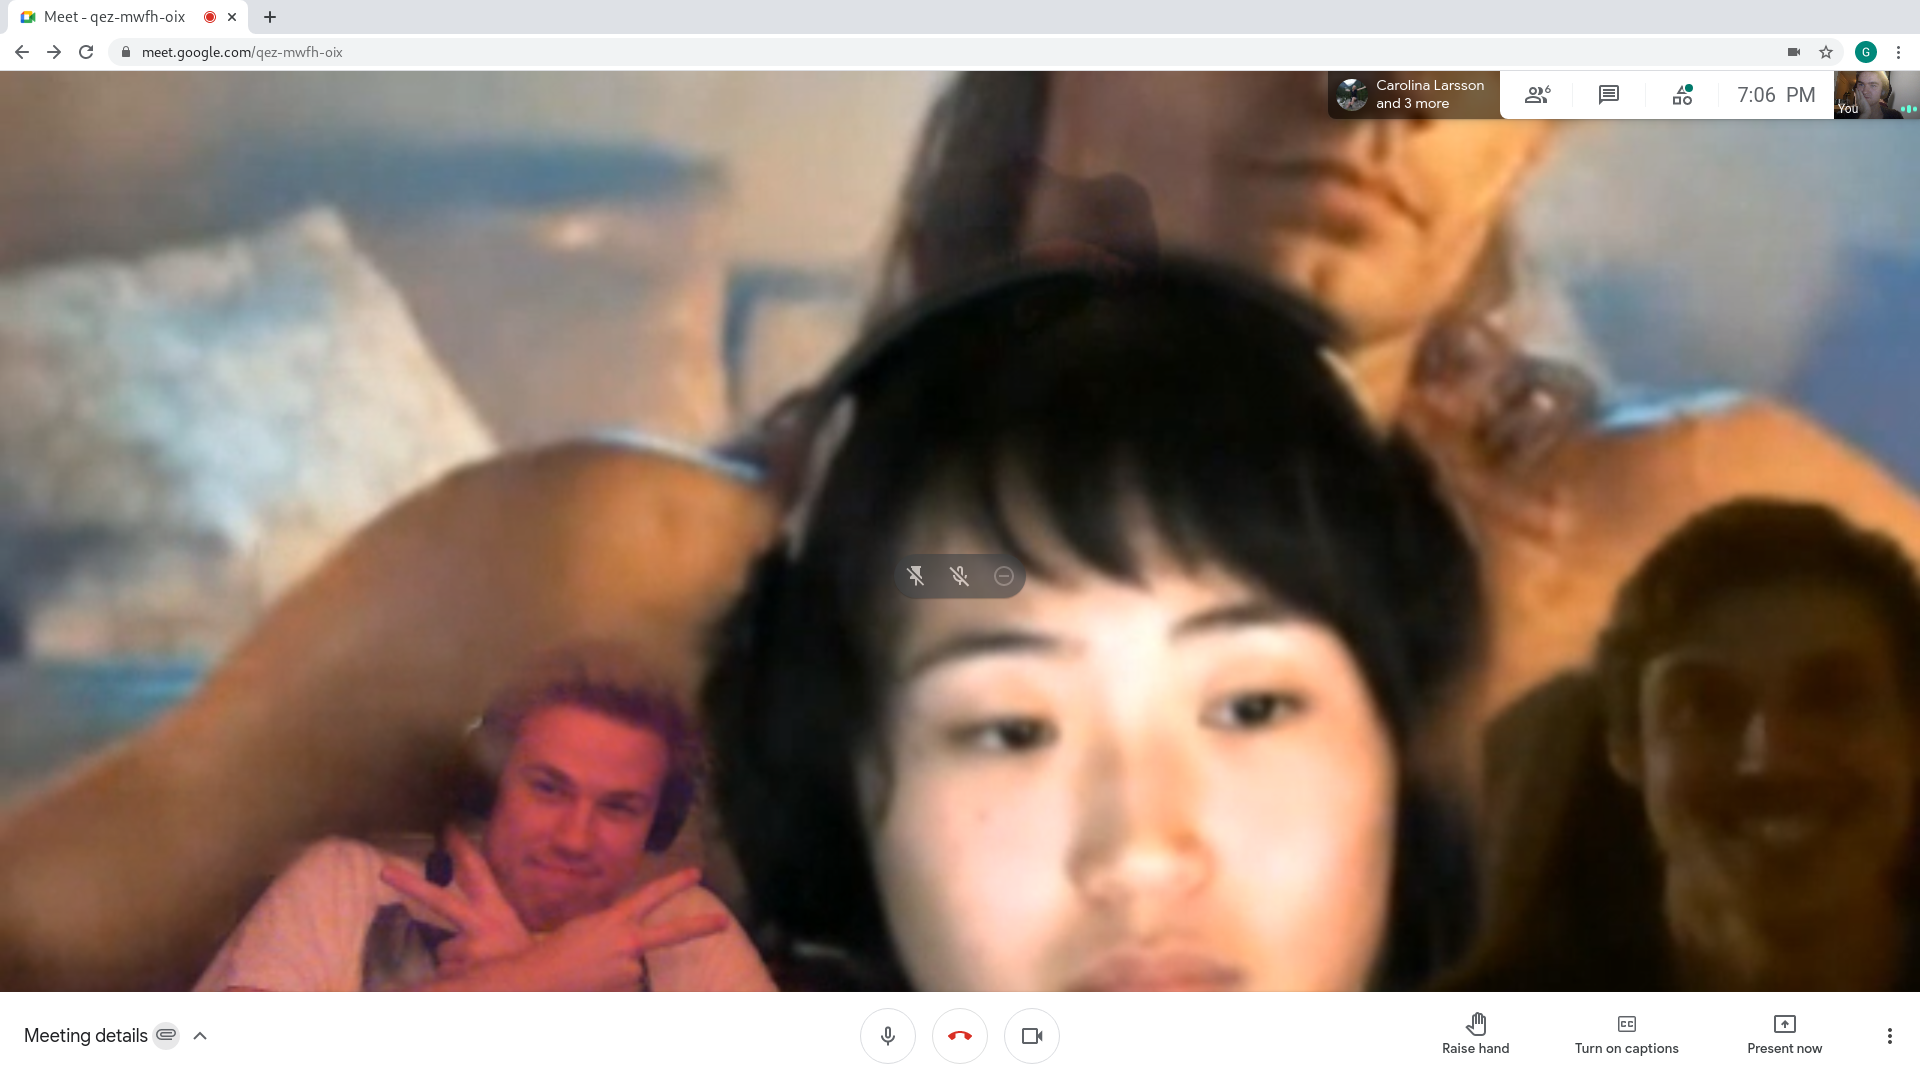
\includegraphics[scale=0.3]{bild.png}
\end{document}